\documentclass[xcolor=dvipsnames,10pt,aspectratio=169]{beamer}
%\documentclass[xcolor=dvipsnames,10pt]{beamer}
\usepackage{etex}
\usepackage{pgf,pgfarrows,pgfnodes,pgfautomata,pgfheaps,pgfshade}
\usepackage[absolute,overlay]{textpos} 
%\usepackage{algorithm}
\usepackage{amsmath,amssymb}
\usepackage[utf8]{inputenc} 
\usepackage{colortbl}
\usepackage{graphicx} 
\usepackage[brazil]{babel}
\usepackage{tabularx} 
\usepackage{multirow}
\usepackage{booktabs}
\usepackage{listings}
\usepackage{multimedia}
\usepackage{animate}
\usepackage{xcolor}
\usepackage{array}
\usepackage{longtable}
\usepackage{makecell}
\usepackage{caption}
\usetheme{Madrid} 

\lstset{ %
%	backgroundcolor=\color{white},   % choose the background color; you must add \usepackage{color} or \usepackage{xcolor}
%	basicstyle=\footnotesize,        % the size of the fonts that are used for the code
	basicstyle=\scriptsize,        % the size of the fonts that are used for the code
	breakatwhitespace=false,         % sets if automatic breaks should only happen at whitespace
	breaklines=true,                 % sets automatic line breaking
	captionpos=t,                    % sets the caption-position to bottom
	commentstyle=\color{mygreen},    % comment style
	deletekeywords={...},            % if you want to delete keywords from the given language
	escapeinside={\%*}{*)},          % if you want to add LaTeX within your code
	extendedchars=true,              % lets you use non-ASCII characters; for 8-bits encodings only, does not work with UTF-8
%	frame=single,                    % adds a frame around the code
	keepspaces=true,                 % keeps spaces in text, useful for keeping indentation of code (possibly needs columns=flexible)
	keywordstyle=\color{blue},       % keyword style
%	language=make,                 % the language of the code
	morekeywords={*,...},            % if you want to add more keywords to the set
%	numbers=left,                    % where to put the line-numbers; possible values are (none, left, right)
%	numbersep=5pt,                   % how far the line-numbers are from the code
	numberstyle=\tiny\color{mygray}, % the style that is used for the line-numbers
	rulecolor=\color{black},         % if not set, the frame-color may be changed on line-breaks within not-black text (e.g. comments (green here))
	showspaces=false,                % show spaces everywhere adding particular underscores; it overrides 'showstringspaces'
	showstringspaces=false,          % underline spaces within strings only
	showtabs=false,                  % show tabs within strings adding particular underscores
	stepnumber=2,                    % the step between two line-numbers. If it's 1, each line will be numbered
}

\definecolor{mygreen}{rgb}{0,0.6,0}
\definecolor{mygray}{rgb}{0.5,0.5,0.5}
\definecolor{mymauve}{rgb}{0.58,0,0.82}

\usecolortheme{beaver}
\newcommand{\ul}{\underline}
\setbeamertemplate{footline}{\scriptsize{\vspace*{0.3cm}\hspace*{15cm}\insertframenumber\,/\,\inserttotalframenumber}}
\setbeamertemplate{caption}[numbered]
\setbeamerfont{caption}{size=\fontsize{8}{5}}

\setbeamercolor{block title}{	bg=Sepia , fg = White}
\setbeamercolor{block body}{bg=Brown!15, fg=Sepia }
\setbeamercolor{item projected}{bg=Sepia, fg=White}
\setbeamercolor{number projected}{bg = Black}

%declara as imagens usadas no layout do slide
\pgfdeclareimage[height=0.8cm]{lmest}{layout_slide/logo_LMest.png}
\pgfdeclareimage[height=0.8cm]{mflab}{layout_slide/logo_mflab_transparente.png}
\pgfdeclareimage[height=1.0cm]{logoufu}{layout_slide/logo_ufu.jpg}
\pgfdeclareimage[height=1.0cm]{petro}{layout_slide/petrobras_2.png}

%posiciona o logotipo do MFLab
\setlength{\TPHorizModule}{1mm}
\setlength{\TPVertModule}{1mm}
\newcommand{\placelogomflab} 
{ 
	\begin{textblock}{13}(150.0,0.0)
		\pgfuseimage{mflab} 
	\end{textblock} 
	
	\begin{textblock}{13}(135.0,0.0)
		\pgfuseimage{lmest} 
	\end{textblock} 
	
% 	\begin{textblock}{13}(128.0,1.0)
% 		\pgfuseimage{logoufu} 
% 	\end{textblock} 
	
	\begin{textblock}{13}(150.0,70.0)
		\pgfuseimage{petro} 
	\end{textblock} 
}
%posiciona o logotipo do MFLab
\setlength{\TPHorizModule}{1mm}
\setlength{\TPVertModule}{1mm}
\newcommand{\placelogo} 
{ 
	\begin{textblock}{13}(150.0,0.0)
		\pgfuseimage{mflab} 
	\end{textblock} 
	
	\begin{textblock}{13}(135.0,0.0)
		\pgfuseimage{lmest} 
	\end{textblock} 
	
% 	\begin{textblock}{13}(128.0,1.0)
% 		\pgfuseimage{logoufu} 
% 	\end{textblock} 
	
	\begin{textblock}{13}(0.0,80.0)
		\pgfuseimage{petro} 
	\end{textblock} 
}

% \setlength{\TPHorizModule}{1mm}
% \setlength{\TPVertModule}{1mm}
% \newcommand{\placelogomflab_titulo} 
% { 
% 	\begin{textblock}{13}(150.0,0.0)
% 		\pgfuseimage{mflab} 
% 	\end{textblock} 
% 	
% 	\begin{textblock}{13}(0.0,0.0)
% 		\pgfuseimage{lmest} 
% 	\end{textblock} 
% 	
% % 	\begin{textblock}{13}(128.0,1.0)
% % 		\pgfuseimage{logoufu} 
% % 	\end{textblock} 
% 	
% 	\begin{textblock}{13}(75.0,80.0)
% 		\pgfuseimage{petro} 
% 	\end{textblock} 
% }



%insere o logotipo da ufu em todos os slides
% \logo{
\includegraphics[height=0.8cm]{figuras/layout_slide/petrobras.png}}

\title{Estudo Dirigido II}

\author{ M.e Hélio Ribeiro Neto \\ \and \\ \and \\ \and \hspace{4cm} Orientador: Prof. Dr. Aristeu da Silveira Neto}

%\date{\tiny{02 de dezembro de 2015}}
\date{\tiny{\today}}
% \newcolumntype{M}[1]{>{\raggedright\arraybackslash}b{#1}}
% \newcolumntype{N}{@{}m{0pt}@{}}	
% \newcolumntype{M}{>{\begin{minipage}[b]{3cm}\raggedright{}}c<{\end{minipage}\minrowheight}}
% \setlength\extrarowheight{5pt}
\newcolumntype{C}[1]{>{\centering\let\newline\\\arraybackslash\hspace{0pt}}m{#1}}


\begin{document}

	\begin{frame}\placelogomflab
		\frametitle 
		{ \vfill
			\centering
			{
			\small{Universidade Federal de Uberlândia}\\
%			\small{Programa de Pós-Graduação em Engenharia Mecânica}\\
			\small{Laboratório de Mecânica dos Fluidos}\\
			}
		}
		\maketitle
	\end{frame}

	\section<presentation>*{Sumário}
	
		\begin{frame}
			\frametitle{Sumário}\placelogomflab 
			{\scriptsize \tableofcontents}
		\end{frame}

		\AtBeginSection[]
		{
		 \begin{frame}<beamer>
		  \frametitle{Sumário}\placelogomflab 
		  {\scriptsize \tableofcontents[current,currentsection]}
		 \end{frame}
		}

		\AtBeginSubsection[]
		{
		 \begin{frame}<beamer>
		  \frametitle{Sumário}\placelogomflab 
		  {\scriptsize \tableofcontents[current,currentsubsection]}
		 \end{frame}
		}

	\section{Movimentação dos pontos lagrangeanos}
	
		\begin{frame}
			\frametitle{Movimentação dos pontos lagrangeanos}
			$\bullet$ Adição da movimentação dos pontos lagrangeanos em função do deslocamento angular da seção transversal.\\
			\centering
			\begin{tabular}{c c}
				
				{\includegraphics[trim=0.0cm 0.0cm 0.0cm 0.0cm,clip=true,loop,height=0.5\textheight]{figuras/rotation_antes.png}}&{\includegraphics[trim=0.0cm 0.0cm 0.0cm 0.0cm,clip=true,loop,height=0.5\textheight]{figuras/rotation_depois.png}}\\
				
			\end{tabular}
		\end{frame}
	
	
		\begin{frame}
			\frametitle{Movimentação dos pontos lagrangeanos}
			\begin{figure}[!ht]
				\centerline{\includegraphics[width=0.3\linewidth]{figuras/rotation_junto.png}}
				\caption{ Comparação }
% 				\label{STDx1}
			\end{figure}

		\end{frame}
	
	\section{ Recálculo das áreas, normais e $\Delta$ s }
	
		\begin{frame}
			\frametitle{Manipulação dos vértices dos triângulos}
			$\bullet$ Antes:\\
				$\longrightarrow$	Todos as contas feitas sobre o centroide do triângulo.\\
				$\longrightarrow$	Área, $\Delta$ s e normais mantidos sem alteração.\\

			$\bullet$ Agora: \\
				$\longrightarrow$ Manipulação dos vértices dos triângulos.\\
				$\longrightarrow$ Recálculo da área, $\Delta$ s e normais a cada passo de tempo.\\
			
		\end{frame}	
		\begin{frame}
			\frametitle{Recálculo das áreas, normais e $\Delta$ s}
			$\bullet$ Adição do recálculo das áreas, normais e $\Delta$ s após a movimentação da estrutura (paralelo).\\

			\begin{figure}[!ht]
				\centerline{\includegraphics[width=\linewidth]{figurasArea.png}}

% 				\label{STDx1}
			\end{figure}


		\end{frame}
	
		\begin{frame}
			\frametitle{Recálculo das áreas, normais e $\Delta$ s}
			$\bullet$ Adição do recálculo das áreas, normais e $\Delta$ s após a movimentação da estrutura (paralelo).\\
			\centering
			\begin{tabular}{c c}
				
				{\includegraphics[width=0.5\linewidth]{figuras/normals.png}}&{\includegraphics[width=0.5\linewidth]{figuras/normals2.png}}

			\end{tabular}
			
			
		\end{frame}
		
	\section{ Adição de fronteiras extras }
		\begin{frame}
			\frametitle{Adição de fronteiras extras}
			$\bullet$ Adição de fronteiras extras.\\
			\begin{tabular}{c c}
				
				{\includegraphics[trim=0.0cm 0.0cm 0.0cm 0.0cm,clip=true,loop,height=0.5\textheight]{figuras/filtration_antes.png}}&{\includegraphics[trim=0.0cm 0.0cm 0.0cm 0.0cm,clip=true,loop,height=0.4\textheight]{figuras/filtration_antes_zoom.png}}\\
				
			\end{tabular}


		\end{frame}
		
		\begin{frame}
			\frametitle{Adição de fronteiras extras}
			\begin{tabular}{c c}
				
				{\includegraphics[trim=0.0cm 0.0cm 0.0cm 0.0cm,clip=true,loop,height=0.5\textheight]{figuras/filtration_depois.png}}&{\includegraphics[trim=0.0cm 0.0cm 0.0cm 0.0cm,clip=true,loop,height=0.4\textheight]{figuras/filtration_depois_zoom.png}}\\
				
			\end{tabular}
			
		\end{frame}
	
	
	\section{ Paralelização e otimização }
		
		\begin{frame}
			\frametitle{Paralelização e otimização}
			$\bullet$ Simplificação e otimização do somatório de forças. (Pedro)\\
			
			$\bullet$ Paralelização do somatório de forças.\\
			
			$\bullet$ Paralelização da movimentação dos pontos lagrangeanos.
			
		\end{frame}
		
		\begin{frame}
			\frametitle{Antes}
			\centering
			\begin{tabular}{c}
				{\includegraphics[width=0.9\textwidth]{figuras/ini.png}}\\{\includegraphics[trim=0.01cm 0.0cm 0.01cm 0.0cm,clip=true,width=0.9\textwidth]{figuras/t_x_51.png}}
			\end{tabular}
	
		\end{frame}

		\begin{frame}
			\frametitle{Antes}
			\centering
			\begin{tabular}{c}
				
				{\includegraphics[trim=0.0cm 0.0cm 0.0cm 0.0cm,clip=true,loop,width=0.9\textwidth]{figuras/sum.png}}\\{\includegraphics[trim=0.01cm 0.0cm 0.01cm 0.0cm,clip=true,loop,width=0.9\textwidth]{figuras/t_x_51f.png}}\\
				
			\end{tabular}
			
		\end{frame}
	
		\begin{frame}
			\frametitle{Antes}
			\centering
			\begin{tabular}{c}
				
				{\includegraphics[trim=0.01cm 0.0cm 0.01cm 0.0cm,clip=true,loop,width=0.9\textwidth]{figuras/t_x_51999.png}}\\ {\includegraphics[trim=0.0cm 0.0cm 0.0cm 0.0cm,clip=true,loop,width=0.9\textwidth]{figuras/adv.png}}
				
			\end{tabular}
			
		\end{frame}
		
		\begin{frame}
			\frametitle{Antes}
			\centering
				\includegraphics[trim=0.0cm 0.0cm 0.0cm 0.0cm,clip=true,loop,width=0.9\textwidth]{figuras/final.png}
		\end{frame}
		
		\begin{frame}
			\frametitle{Agora}
			\centering
			{\includegraphics[trim=0.0cm 0.0cm 0.0cm 0.0cm,clip=true,loop,width=0.85\textwidth]{figuras/ini.png}}
			\begin{tabular}{c}
				
				{\includegraphics[trim=0.00cm 2.0cm 0.0cm 2.0cm,clip=true,loop,width=0.85\textwidth]{figuras/t_x_51.png}}\\{\includegraphics[trim=0.00cm 2.0cm 0.0cm 2.0cm,clip=true,loop,width=0.85\textwidth]{figuras/t_x_51f.png}}\\{\includegraphics[trim=0.00cm 2.0cm 0.0cm 2.0cm,clip=true,loop,width=0.85\textwidth]{figuras/t_x_51fg.png}}\\{\includegraphics[trim=0.00cm 2.0cm 0.0cm 2.0cm,clip=true,loop,width=0.85\textwidth]{figuras/t_x_51fy.png}}\\{\includegraphics[trim=0.00cm 2.0cm 0.0cm 2.0cm,clip=true,loop,width=0.85\textwidth]{figuras/t_x_51fb.png}}\\
				
			\end{tabular}
			
		\end{frame}
		
		\begin{frame}
			\frametitle{Agora}
			\centering
			\begin{tabular}{c}
				
				{\includegraphics[trim=0.00cm 2.0cm 0.0cm 2.0cm,clip=true,loop,width=0.9\textwidth]{figuras/t_x_51f.png}}\\{\includegraphics[trim=0.01cm 0.0cm 0.01cm 0.0cm,clip=true,loop,width=0.9\textwidth]{figuras/t_x_51999.png}}\\{\includegraphics[trim=0.01cm 0.0cm 0.01cm 0.0cm,clip=true,loop,width=0.9\textwidth]{figuras/t_x_51999g.png}}\\{\includegraphics[trim=0.01cm 0.0cm 0.01cm 0.0cm,clip=true,loop,width=0.9\textwidth]{figuras/t_x_51999y.png}}\\{\includegraphics[trim=0.01cm 0.0cm 0.01cm 0.0cm,clip=true,loop,width=0.9\textwidth]{figuras/t_x_51999b.png}}
				
			\end{tabular}
			
		\end{frame}

		
		\begin{frame}
			\frametitle{Agora}
			\centering
			\includegraphics[trim=0.0cm 0.0cm 0.0cm 0.0cm,clip=true,loop,width=0.9\textwidth]{figuras/final.png}

		\end{frame}
		
		\section{ Arquivos de saída da fronteira}
		\begin{frame}
			\frametitle{Malha não estruturada para visualização vtp, pvtp e pvd}
			
			$\bullet$ Antes:\\
			$\longrightarrow$	Todos as contas feitas sobre o centroide do triângulo;\\
			$\longrightarrow$	Escrita em serial;\\
			$\longrightarrow$	Centroides e propriedades dos centroides;\\
			$\longrightarrow$	Visualização em forma de Glyph (esferas) ou Delaunay (caro e erro);\\
			$\longrightarrow$	Escrita em vtk DataFile Version 2.0 (formato antigo);\\
			$\longrightarrow$	Escrita em ASCII; \\
			\\ 
			$\bullet$ Agora: \\
			$\longrightarrow$ Manipulação dos vértices dos triângulos;\\
			$\longrightarrow$ Escrita em paralelo;\\
			$\longrightarrow$ Malha não estruturada com propriedades de célula;\\
			$\longrightarrow$ Visualização automática da malha;\\
			$\longrightarrow$ XML File Formats (formato novo em paralelo);\\
			$\longrightarrow$ Escrita em binário;
			
		\end{frame}
	
		\section{Acoplamento Fraco}
		\begin{frame}
			\frametitle{Acoplamento Fraco}
			\includegraphics[trim=0.0cm 0.0cm 0.0cm 0.0cm,clip=true,loop,width=0.9\textwidth]{figuras/fraco.png}
	
		\end{frame}
	
		\section{Acoplamento Forte no MFSim}
		
		
		\begin{frame}
			\frametitle{Gauss-Seidel ou Iteração de ponto fixo}
			\centering
		   \begin{equation}\label{forte_eq}
				F = Fluido(D)
			\end{equation}
		   \begin{equation}\label{forte_eq2}
				D = Estrutura(F)
			\end{equation}
		   \begin{equation}\label{forte_eq3}
			  K(D) =  Estrutura(Fluido(D))-D =  0
			\end{equation}
			
			\flushleft

			Expansão em série de Taylor da função $K(D+\Delta D)$ e truncando no termo de primeira ordem:
			\begin{equation}\label{forte_eq4}
			K(D+\Delta D) \approx K(D)
			\end{equation}
			\centering
			\begin{equation}\label{forte_eq5}
			K(D_0) = res
			\end{equation}
			\flushleft
			Quando $res$ for menor que uma tolerância tem-se a solução do sistema não linear. Para a próxima iteração do solver faz-se:
			
			\centering
			\begin{equation}\label{forte_eq6}
			D_1 = D_0 + \omega \, res
			\end{equation}
			\flushleft
			 No MFSim está implementada a avaliação dinâmica de Aitken $\delta^2$\\
			
		\end{frame}
	

		\begin{frame}
			\frametitle{Newton-Raphson}
			\flushleft
			Expansão em série de Taylor da função $K(D+\Delta D)$ e truncando no termo de segunda ordem:
			
			\centering
			\begin{equation}\label{forte_eq_Newton}
			K(D+\Delta D) \approx K(D)+\Delta D \, J(D)
			\end{equation}
			\begin{equation}\label{forte_eq_Newton2}
			\Delta D \approx -K(D)J(D)^{-1}
			\end{equation}
			
			\flushleft
			$J(D)$ deve ser quadrada:
			
			\centering
			\begin{equation}\label{forte_eq_Newton3}
			K: \mathbb{R}^{n} \to \mathbb{R}^{n}
			\end{equation}
			
			\flushleft
			$J(D)$ é de tamanho $n \, x \, n$.
		\end{frame}
		
		
		\begin{frame}
			\frametitle{Newton-Raphson}
			
			\flushleft
			Método de interface com jacobiano composto:
			
			\centering
			\begin{equation}\label{forte_eqNewton}
			K(D+\Delta D) \approx K(D)+\Delta D \, J(D)
			\end{equation}
			\begin{equation}\label{forte_eqNewton2}
			K(D) =  Estrutura(Fluido(D))-D =  0
			\end{equation}
			\begin{equation}\label{forte_eqNewton3}
			J(D) =  Estrutura'(Fluido(D)) \, Fluido'(D)-I
			\end{equation}
			\begin{equation}\label{forte_eqNewton4}
			Fluido(D): \mathbb{R}^{n} \to \mathbb{R}^{m}
			\end{equation}
			
			\flushleft
			$Fluido'(D)$ é de tamanho $m x n$
			
			\centering
			
			\begin{equation}\label{forte_eqNewton5}
			Estrutura(F): \mathbb{R}^{m} \to \mathbb{R}^{n}
			\end{equation}
			
			\flushleft
			$Estrutura'(F)$ é de tamanho $n x m$\\
			$Estrutura'(Fluido(D)) \, Fluido'(D)$ e $I$ é de tamanho $n x n$
		\end{frame}
	
		\begin{frame}
			\frametitle{Quasi-Newton-Raphson}
				
				\flushleft
				Os métodos implementados no MFsim são:
				
				$\bullet$ Primeiro método de Broyden; (Jacobiano e Inversa)
				
				$\bullet$ Segunda método de Broyden;(Inversa)
				
				$\bullet$ Método de McCormick;(Inversa)
				
				$\bullet$ Método de Davidon-Fletcher-Powell (DFP);(Inversa)
				
				$\bullet$ Método de Broyden-Fletcher-Goldfarb-Shanno (BFGS);(Inversa)
				
				$\bullet$ Método de Greenstadt.(Inversa)
		\end{frame}
		
		
		\begin{frame}
			\frametitle{Conveniência do método de Multi Direct Forcing}
			
			\flushleft
			\textbf{Fraco:}\\
			$\bullet$ Predição da velocidade.\\
			$\bullet$ MDF. (Imposição da condição de dirichlet na interface e cálculo da força)\\
			$\bullet$ Estrutura.\\
			$\bullet$ Poisson.\\
			$\bullet$ Correção de velocidade e pressão.\\ \\

			\textbf{Forte:}\\
			$\bullet$ Predição da velocidade.\\
			while \\
			\quad	$\longrightarrow$ MDF.\\
			\quad	$\longrightarrow$ Estrutura.\\
			end\\
			$\bullet$ Poisson.\\
			$\bullet$ Correção de velocidade e pressão.\\

		\end{frame}
		
		\section{Resultados}
		\begin{frame}
		\frametitle{Limite do fraco}
			ct=121
			mi=200
			\begin{tabular}{c c}
			{\includegraphics[width=0.45\linewidth]{../../simulacoes_Estudo_dirigido2/fraco_mi_200_0_15_ct141/figuras/estrutura/vel_151}}&
		   {\includegraphics[width=0.45\linewidth]{../../simulacoes_Estudo_dirigido2/fraco_mi_200_0_15_ct141/figuras/estrutura/vel_251}}\\
		   {(a) Velocidade em linha centro da estrutura} & {(b) Velocidade transversal centro da estrutura}
		\end{tabular}
		\end{frame}
		
		\begin{frame}
		\frametitle{Limite do fraco}
			ct=121
			mi=250
			\begin{tabular}{c c}
				{\includegraphics[width=0.45\linewidth]{../../simulacoes_Estudo_dirigido2/fraco_mi_250_0_2_ct121/figuras/estrutura/vel_151}}&				
				{\includegraphics[width=0.45\linewidth]{../../simulacoes_Estudo_dirigido2/fraco_mi_250_0_2_ct121/figuras/estrutura/vel_251}}\\
				{(a) Velocidade em linha centro da estrutura} & {(b) Velocidade transversal centro da estrutura}
			\end{tabular}
		\end{frame}
	
		\begin{frame}
		\frametitle{Limite do fraco}
			mi=250
			\begin{tabular}{c c}
				{\includegraphics[width=0.5\linewidth]{../../simulacoes_Estudo_dirigido2/figuras_comparacoes/mdf_tempo_fraco/estrutura/v_x_151}}&{\includegraphics[width=0.5\linewidth]{../../simulacoes_Estudo_dirigido2/figuras_comparacoes/mdf_tempo_fraco/estrutura/v_x_251}}\\
				{(a) Velocidade em linha centro da estrutura} & {(b) Velocidade transversal centro da estrutura}
			\end{tabular}
		\end{frame}
		
		
		\begin{frame}
			\frametitle{Forte e influencia do tempo de início}
			mi=10
			\begin{tabular}{c c}
				{\includegraphics[width=0.5\linewidth]{../../simulacoes_Estudo_dirigido2/figuras_comparacoes/mdf_tempo/estrutura/v_x_151}}&{\includegraphics[width=0.5\linewidth]{../../simulacoes_Estudo_dirigido2/figuras_comparacoes/mdf_tempo/estrutura/v_x_251}}\\
				{(a) Velocidade em linha centro da estrutura} & {(b) Velocidade transversal centro da estrutura}
			\end{tabular}
		\end{frame}
	
		\begin{frame}
			\frametitle{Tempo de início e força}
			mi=10
			\begin{tabular}{c c}
				{\includegraphics[width=0.5\linewidth]{../../simulacoes_Estudo_dirigido2/figuras_comparacoes/mdf_tempo/estrutura/f_x_251}}&{\includegraphics[width=0.5\linewidth]{../../simulacoes_Estudo_dirigido2/figuras_comparacoes/mdf_tempo/estrutura/f_x_451}}\\
				{(a) Força em linha centro da estrutura} & {(b) Força transversal centro da estrutura}
			\end{tabular}
		\end{frame}
	
		\begin{frame}
			\frametitle{Tempo de início e força}
			mi=10
			\begin{tabular}{c c}
				{\includegraphics[width=0.5\linewidth]{../../simulacoes_Estudo_dirigido2/figuras_comparacoes/mdf_tempo/estrutura/f_x_151}}&{\includegraphics[width=0.5\linewidth]{../../simulacoes_Estudo_dirigido2/figuras_comparacoes/mdf_tempo/estrutura/f_x_351}}\\
				{(a) Força em linha centro da estrutura} & {(b) Força em linha centro da estrutura}
			\end{tabular}
		\end{frame}
		
		\begin{frame}
		\frametitle{MDF fixo e variável}
		mi=10
		\begin{tabular}{c c}
				{\includegraphics[width=0.5\linewidth]{../../simulacoes_Estudo_dirigido2/figuras_comparacoes/mdf_fixo/estrutura/v_x_251}}&{\includegraphics[width=0.5\linewidth]{../../simulacoes_Estudo_dirigido2/figuras_comparacoes/mdf_fixo/estrutura/f_x_151}}\\
				{(a) Força transversal centro da estrutura} & {(b) Força transversal centro da estrutura}
			\end{tabular}
		\end{frame}
	
		\begin{frame}
			\frametitle{Influência da malha}

			\begin{tabular}{c c}
				{\includegraphics[width=0.65\linewidth]{figuras/area2}}&{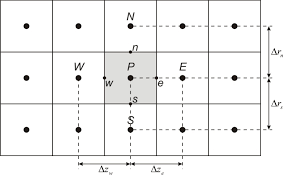
\includegraphics[width=0.3\linewidth]{figuras/malha}}
			\end{tabular}
		\end{frame}
	
		\begin{frame}
			\frametitle{Influência da malha}
			mi=10
			\begin{tabular}{c c}
				{\includegraphics[width=0.5\linewidth]{../../simulacoes_Estudo_dirigido2/figuras_comparacoes/malha/estrutura/v_x_151}}&{\includegraphics[width=0.5\linewidth]{../../simulacoes_Estudo_dirigido2/figuras_comparacoes//malha/estrutura/v_x_251}}\\
				{(a) Velocidade em linha centro da estrutura} & {(b) Velocidade transversal centro da estrutura}
			\end{tabular}
		\end{frame}	
	
		\begin{frame}
			\frametitle{Comparação número de iterações}
			\begin{tabular}{c c c c}
				\hline
				Método & Mínimo     &    Máximo &  Média\\ \hline
				FPI MDF variável & 8     &    101 &  8.9764764764764760\\
				FPI MDF fixo & 8     &     11 &  8.9099099099099099\\
				QN Primeiro método de Broyden MDF variável & 18    &     101 &  18.281281281281281 \\ \hline
			\end{tabular}
		\end{frame}	
	
		\begin{frame}
			\frametitle{Perspectivas}
			$\bullet$ Extrapolação temporal para chute inicial do acoplamento forte;\\
			$\bullet$ Spool no AMR;\\
			$\bullet$ Validação do acoplamento forte;\\
			$\bullet$ Outro método de fronteira imersa (Ghost Fluid);\\
			$\bullet$ Estimativa do Jacobiano via mínimos quadrados;\\
			$\bullet$ Fluido-estrutura monolítico:\\
			$\longrightarrow$ Fluido monolítico;\\
			$\longrightarrow$ Ghost Fluid monolítico;\\
			$\longrightarrow$ Modelo de turbulência monolítico;\\
			$\longrightarrow$ Estrutura monolítico.\\
		\end{frame}	
	
		\section{Agradecimentos}
			\begin{frame} %\placelogomflab 
				\placelogomflab 
				\frametitle{Agradecimentos}
				\begin{figure}
					\begin{center}
						\begin{tabular}{c c}
							{
\includegraphics[trim=0.0cm 0.0cm 0.0cm 0.0cm,clip=true,loop,height=0.2\textheight]{layout_slide/petrobras.png}}&{\includegraphics[trim=0.0cm 0.0cm 0.0cm 0.0cm,clip=true,loop,height=0.2\textheight]{layout_slide/logo_mflab.png}}\\
							{\includegraphics[trim=0.0cm 0.0cm 0.0cm 0.0cm,clip=true,loop,height=0.2\textheight]{layout_slide/cnpq.png}}&{\includegraphics[trim=0.0cm 0.0cm 0.0cm 0.0cm,clip=true,loop,height=0.2\textheight]{layout_slide/CAPES.png}}\\
							{\includegraphics[trim=0.0cm 0.0cm 0.0cm 0.0cm,clip=true,loop,height=0.2\textheight]{layout_slide/FAPEMIG.jpg}}&{\includegraphics[trim=0.0cm 0.0cm 0.0cm 0.0cm,clip=true,loop,height=0.2\textheight]{layout_slide/UFU_black.jpg}}\\
						\end{tabular}
					\end{center}
				\end{figure}
			\end{frame}
			
			\begin{frame} %\placelogomflab 
				\placelogomflab 
				\frametitle{Agradecimentos}
				\fontsize{44pt}{7.2}\selectfont
				\begin{center}
					Obrigado.
				\end{center}
			\end{frame}
		
\end{document}
